\documentclass[10pt]{article}

% dependencies
\usepackage{multirow} % better tables
\usepackage{enumitem} % better lists
\usepackage{array,ragged2e} % better tables: alignment
\usepackage{amsmath, mathtools} % better equations: text
\usepackage[makeroom]{cancel} % better equations: strikethrough
\usepackage[ruled,vlined]{algorithm2e} % algorithms
\usepackage[pdfusetitle]{hyperref} % for links and PDF metadata
\usepackage{makecell} % better tables: multi-line cells
\usepackage[backend=biber,style=ieee]{biblatex} % bibliography
\usepackage{geometry} % margin control
\usepackage{graphicx} % include images
\usepackage{float} % for table and figure placement

% configuration
\setlength\parindent{0pt} % NO indents
\addbibresource{references.bib} % references
\geometry{margin=1.5in} % 1.5inch margins
\graphicspath{ {images/} } % image folder

% metadata
\title{Reinforcement Learning in Minesweeper}
\date{April 12, 2021}
\author{Dudhat, Hird, Kosman, Theriault, White, Zhao}

% document
\begin{document}
\makeatletter
\newcommand\authors[1]{\renewcommand\@authors{#1}}
\newcommand\@authors{\@latex@error{No \noexpand\author given}\@ehc}
\makeatother

\authors{
  \makecell[tc]{
    \textbf{Janhavi Dudhat}\\
    Computer Science\\
    University of Victoria\\
    \emph{janhavidudhat@uvic.ca}
  } & \makecell[tc]{
    \textbf{Nick Hird}\\
    Computer Science\\
    University of Victoria\\
    \emph{nicholash@uvic.ca}
  } \\ \makecell[tc]{
    \textbf{Sam Kosman}\\
    Software Engineering\\
    University of Victoria\\
    \emph{skosman@uvic.ca}
  } & \makecell[tc]{
    \textbf{Scott Theriault}\\
    Software Engineering\\
    University of Victoria\\
    \emph{scottlt@uvic.ca}
  } \\ \makecell[tc]{
    \textbf{Zak White}\\
    Computer Science\\
    \& Statistics\\
    University of Victoria\\
    \emph{zakerywhite@uvic.ca}  
  } & \makecell[tc]{
    \textbf{Yichun Zhao}\\
    Computer Science \&\\
    Health Information Science\\
    University of Victoria\\
    \emph{yichunzhao@uvic.ca}
  }
}

\def\arraystretch{2.5}
\makeatletter
\noindent\makebox[\textwidth]{
  \begin{minipage}{1.25\textwidth}
    \centering
    \rule{\textwidth}{2pt}\\
    \vspace{5mm}
    {\Huge \@title}\\
    \vspace{3mm}
    \rule{\textwidth}{1pt}
    \begin{tabular}[t]{cc}%
      \@authors
    \end{tabular}
  \end{minipage}
}
\makeatother
\def\arraystretch{1}

\vspace{2cm}

\begin{center}
    \begin{minipage}{0.75\textwidth}
    \begin{center}\section*{Abstract}\end{center}
    Minesweeper is a famous puzzle game involving a single player, requiring them to clear a board with hidden mines and numerical clues indicating the number of mines in the neighbourhood. We have implemented the Q learning and deep Q learning algorithms, ran several experiments on the reward structures, tuned hyperparameters, trained two final agents, and achieved different levels of success. Both the agents performed substantially better than a baseline random agent. Given the limitation of training time, the Q learning agent performed better in average reward and board completion rate, but the deep Q learning agent had a higher winning rate. The latter is likely to perform better if trained for longer, and is ultimately better suited for larger boards with continuous state spaces due to its ability to predict best actions for unseen states.
    \end{minipage}
\end{center}

\thispagestyle{empty}
\section{Introduction}

Minesweeper is a puzzle game with the objective of clearing a rectangular board of hidden mines. 
For each move, the player chooses one cell on the board, revealing either a mine or information about adjacent cells.
The player either wins when all unopened cells contain mines, or loses after revealing a mine.
The game of Minesweeper is NP-complete \cite{kaye}, meaning it is possible to implement a brute-force solver. 
Despite this possibility, a more interesting approach to solving the game is using machine learning.
Our objective is to develop Minesweeper solvers using Q-learning and deep Q-learning.

\section{Problem}

The problem is to develop a Q-learning and deep Q-learning agent to play the game  Minesweeper. Due to the nature of reinforcement learning, datasets cannot be used for this purpose. Instead, a Minesweeper gym environment was developed to train our agent to allow for the selection of actions.
\\\\
Minesweeper, as a puzzle game, involves logic, strategies, and pattern recognition. By training an agent to solve games, we can observe which decisions the agent makes based on patterns humans may not be able to notice or understand. 

\subsection{Approach}

We configured a training environment to simulate Minesweeper games. Then, the Q learning algorithm is implemented, and the Q-learning agent is trained with different reward structures. After finding the most suitable structure that provides the best results, hyperparameters are tuned over approximately 8 million games. Due to the high number of possible states, we only trained our agent for a small board size of $4\times4$. To demonstrate the agent’s learning, its performance was then evaluated against the performance of an agent that made randomly generated moves.
\\\\
After observing the results of the Q-learning agent, we implemented and trained a deep Q-learning agent by using the same optimal hyperparameter values and the Deep Reinforcement Learning Library (keras-rl2).

\subsection{Goals}

We will measure the success of our agent by its ability to win randomly-generated games.
To measure progression, we will track the win rate, board completion, and average total reward as the agent is trained, then evaluate the same metrics on the fully-trained agent to quantify its success.
\\\\
We also ran an untrained agent to collect the win rates of randomly generated moves; and compared our results with this. Our goal was to at least beat the scores of this untrained agent; a larger the difference in the win rates would prove our agent has learnt more.

\section{Related Work}

In our initial research, we discovered several reports describing various approaches to solving Minesweeper.
Gardea, Koontz, and Silva achieved up to a win rate of 32\% using a combination of logistic regression, support-vector machines, and simplified Q-learning \cite{gardea}.
Most inspirationally, Stephen Lee outlined his approach to configuring a deep Q-learning agent that reached an 80\% win rate after training \cite{lee}. 
Previous attempts using simple Q-Learning have failed to achieve win rates of greater than 5\% with board sizes upwards of $6\times6$ \cite{mehta}, which factored into our decision to limit the problem to a $4\times4$ board.

\section{Environment}
Because of the nature of the problem, we cannot use pre-existing datasets to train the agent. 
Rather, we configured a training environment to simulate Minesweeper games. In the environment,
\begin{itemize}
  \item a game represents an \textbf{episode},
  \item the board represents the \textbf{state}, and
  \item each possible move represents an \textbf{action}.
\end{itemize}
The first environment we used was a naive implementation, containing a basic 2D matrix representing the game board.
Each matrix value contained one of: a number from 0 to 8, corresponding to the number of adjacent mines; a $-$2, indicating an unopened cell; or $-$1, a mine.
The scope of possible actions is any cell -- imposing the possibility of selecting a previously-opened cell.
Because of this flaw, and the lack of penalization for repeated actions, the agent would often get stuck and fail to learn.
\\\\
A more advanced environment was implemented, restricting valid actions to only unopened cells.
The new environment also opens neighbouring cells when a safe cell is selected, in accordance with the real Minesweeper game.
These changes drastically reduced the number of steps taken to complete a game, making training both more efficient and more effective.
Additionally, in the new environment, if the first opened cell reveals a mine, the game will silently restart to avoid failing on the first move and not learning. 
This advanced environment was configured for use with both Q-learning and deep Q-learning.

\subsection{Reward Structure}
The initial reward structure (Structure 1) was brainstormed. Initially, the positively rewarded actions were winning a game, and opening a new cell and losing the game was a negative reward. When using such a simple reward structure with our very first environment (the most naive Gym environment), we found that even after 1000 runs, the agent failed to learn to not click on an already opened cell. This made sense as the reward structure was flawed, since reopening a cell would still result in the agent being positively rewarded. Hence, in our next version of the reward structure (Structure 2), we gave a negative reward to the agent for clicking on the already opened cell, and kept everything else the same as Structure 1.
\\\\
A more advanced reward structure (Structure 3) was then adapted to have the agent rewarded positively for winning and opening a new cell (strategically, based on what the agent has learnt so far). Structure 3 rewarded the agent negatively for guessing which cell to open, reopening an open cell, and losing.
\\\\
We did some research by actually playing the Minesweeper game, and observing someone who has never played the game to devise reward strategies that would help an agent learn more effectively. Based on that, we designed a new reward structure (Structure 4). Here, the agent was rewarded like in Structure 2, except in Structure 2 the reward for opening a new cell was a constant whereas in Structure 4, we decided to take a dynamic approach for opening a new cell. The new reward for opening a new cell was based on the percentage of new cells opened by the action - an action that chose a cell adjacent to a mine would be rewarded less than an action that would open neighbouring cells.
\\\\
Table 1 states the reward values for each action. The values are consistent throughout all four reward structures, except for the opening a cell action in Structure 4.

\begin{table}[h]
  \centering
  \begin{tabular}[t]{| l | c |}
    \hline
    \textbf{Action} & \textbf{Reward}\\
    \hline
    Opening a new cell \ \ & +0.3 \\
    Reopening a cell & -0.3 \\
    Guessing a cell & -0.3 \\
    Victory & +1.0 \\
    Loss & -1.0 \\
    \hline
  \end{tabular}
  \caption{Reward summary}
\end{table}


\subsubsection{Comparing Reward Structures}

We excluded Structure 1 from our tests, since we had already established the poor performance of the agent using that structure. 
\\\\
To compare the three remaining structures, we tested multiple episodes on different board sizes (Appendix A). The performance is judged based on the percentage of games won during testing. The overall results pointed towards the comparatively worse performance of Structure 4. However, the performance of Structure 2 and Structure 3 were relatively close.
\\\\
To further obtain the best structure to use, we compared Structure 2 and Structure 3. This time, we used a bigger board and more episodes for a deeper comparison. The results, as seen in the figures below, manifest that the agent trained with Structure 2 (which is one step simpler than Structure 3) was able to win a higher percentage of games consistently, even though not by a substantial difference. This could potentially mean that Structure 3 is overcomplicating the reward structure, and trying harder to control the agent does not lead to better results.

\begin{figure}[H]
\centering
\makebox[\textwidth]{
	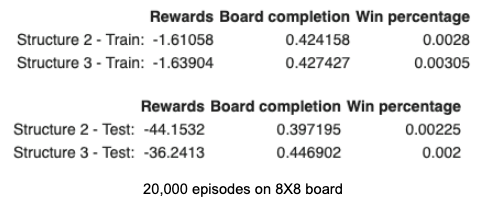
\includegraphics[width=0.55\textwidth]{reward-20k.png}
	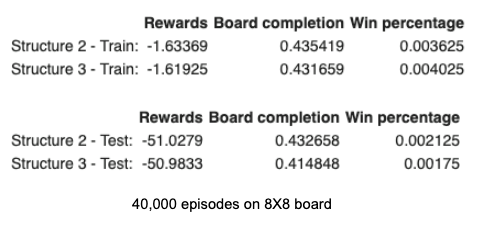
\includegraphics[width=0.55\textwidth]{reward-40k.png}
}
\caption{Comparison of Structure 2 and Structure 3}
\end{figure}

Since Structure 2 performed better when tested, we chose to train our Q-learning and deep Q-learning agents using this structure. Recall that this structure positively rewarded for winning (+1) and opening a new cell (+0.3), and negatively rewarded for losing (-1) and reopening an already opened cell (-0.3).

\section{Q-Learning}
The implementation of Q-learning involves the construction of a Q-table which holds a Q-value for each pairwise combination of states and actions.
For any state, the action that provides the maximum Q-value for that state in the table represents the best possible action.
After each action, the corresponding Q-value is updated by using the Bellman equation \cite{mitchell}:

\setlength\parindent{15pt}
\[
 \underbrace{Q'(s,a)}_{\mathclap{\substack{\text{New Q-value} \\ \text{for this state} \\ \text{and action}}}} 
  = \overbrace{Q(s,a)}^{\mathclap{\substack{\text{Current} \\ \text{Q-value}}}} 
  + \underset{\mathclap{\substack{\\ \uparrow \\ \text{Learning} \\ \text{rate}}}}{\alpha}
  [ \overbrace{R(s,a)}^{\mathclap{\substack{\text{Reward for} \\ \text{this state} \\ \text{and action}}}} 
  + \overset{\mathclap{\substack{\text{\indent\indent  Discount} \\ \text{\indent\indent rate} \\ \indent\swarrow \\ \text{}}}}{\gamma} 
  \underbrace{maxQ(s',a')}_{\mathclap{\substack{\text{Maximum future reward} \\ \text{for all possible actions} \\ \text{at the new state}}}}
  - Q(s, a)] 
\]
\setlength\parindent{0pt}

The agent learns through a combination of exploitation and exploration: choosing the best possible action using the Q-table, or choosing a random action, respectively.
During training, the decision between exploration and exploitation is dictated by the exploration parameter ($\epsilon$), representing the chance an action is explorative. 
At each step, the exploration rate is reduced to progressively reduce the amount of random actions taken.
The basic pseudocode for the algorithm is defined below \cite{mateo}.
\\

\begin{algorithm}[H]
  \caption{Q-Learning} 
  \SetAlgoLined
  Parameters: $\epsilon, \alpha, \gamma \in (0, 1]$\;
  \For{each episode}{
    Initialize state $S$\;
    \While{game is not over}{
      Choose $A$ from $S$ using exploitation or exploration\;
      Take action $A$, observe state $S'$ and reward $R(S, A)$\;
      $Q(S, A) \leftarrow$ new Q-value computed with the Bellman equation\;
      $S \leftarrow$ S'\;
    }
    Reduce exploration rate\;
  }
\end{algorithm}

\subsection{Hyperparameter Tuning}
Once the Q-learning was implemented, we began tuning each of four hyperparameters to optimize the agent's results. To do this, a range of values was created for each parameter. Then, for each varied parameter value, a $4\times4$ board was used to run the agent for 40,000 episodes for training. The training’s generated Q-table was then used for testing over 8000 episodes. Within each round the score, win percentage, and board completion was recorded in order to be graphed against the parameter. Using these graphs (included in Appendix B), the optimized hyperparameter was selected. 

\begin{itemize}
  \item {
    The \textbf{discount rate}, $\gamma \in (0, 1]$\\
    The discount rate quantifies the importance of future rewards -- a smaller value prioritizes immediate rewards, while a higher value places emphasis on future rewards. 
    There was a slight increase in win percentage as discount rate increased, with 0.90 giving the highest test win rate. 
    At 0.90, the agent will heavily consider future rewards over immediate rewards.
    
  }
  \item {
    The \textbf{learning rate}, $\alpha \in (0, 1]$\\
    The learning rate dictates to what extent newly-learnt information overrides existing information.
    With the best value of 0.05, the agent relies heavily on prior knowledge, learning very little for each step.
    
  }
  \item {
    The \textbf{minimum exploration rate}, $\epsilon_{min} \leq 0.1$\\
    As the exploration rate decays, $\epsilon_{min}$ controls the limit of exploitation. 
    The smaller the value, the less exploration will occur as the agent progresses through training.  
    There was a steady decline in win rate as $\epsilon_{min}$ increased, so we selected a small value of 0.005.
  }
  \item {
    The \textbf{exploration decay rate}, $\epsilon_{decay} \leq 0.02$\\
    The epsilon decay rate defines how much the exploration rate will decrease after each episode.
    The win percentage remained mostly uniform as $\epsilon_{decay}$ grew, but peaked when at 0.01, resulting in a gradual exploration decay.
  }
\end{itemize}

\begin{table}[H]
  \centering
  \begin{tabular}[t]{| r | c | c |}
    \hline
    \multicolumn{2}{|c|}{\textbf{Hyperparameter}} & \textbf{Value} \\
    \hline
    Discount rate & $\gamma$ & 0.9 \\
    Learning rate & $\alpha$ & 0.05 \\
    Min. exploration rate & $\epsilon_{min}$ & 0.005\\
    Exploration decay rate & $\epsilon_{decay}$ & 0.01\\
    \hline
  \end{tabular}
  \caption{Hyperparameter value summary}
\end{table}

\subsection{Results}

Agents were trained and tested using the Q-learning algorithm for various numbers of episodes, the results of which are summarized in Table 3.

\begin{table}[H]
  \centering
  \begin{tabular}[t]{| l | l | l | c | c |}
    \hline
    \multicolumn{2}{|c|}{\textbf{Agent}} & \textbf{Episodes} & \textbf{Win Rate} & \textbf{Score} \\
    \hline
    \multirow{2}{*}{1} & Train & 500,000 & 11.8512 & 0.2919 \\
    & Test & 1,000 & 13.9 & 0.6426 \\
    \hline
    \multirow{2}{*}{2} & Train & 1,000,000 & 15.1084 & 0.4393 \\
    & Test & 2,000 & 17.1 & 0.63118 \\
    \hline
    \multirow{2}{*}{3} & Train & 4,000,000 & 13.2549 & 0.5456 \\
    & Test & 1,000,000 & 14.0274 & 0.62 \\
    \hline
    \multirow{3}{*}{4} & Train & 7,984,000 & 13.3 & 0.5352 \\
    & Test & 16,000 & 13.5375 & 0.5712 \\
    & Test & 1,996,000 & 13.6519 & 0.5725 \\
    \hline
  \end{tabular}
  \caption{Q-learning results summary}
\end{table}



The final test agent (Agent 4 tested with 1,996,000 episodes) achieved a board completion of 58.4\%.
As the number of training episodes increases, the agent seems to approach a win-rate in the 13\% to 14\% range. Looking at the testing results, the agents do not show evidence of overfitting, and thus could be further trained to theoretically increase their accuracy. 
\section{Deep Q-Learning}
\subsection{Motivation}
The greatest constraint of the Q-learning implementation is the spatial complexity of the \emph{Q-table}. 
The maximum size of the \emph{Q-table} is the product of possible states and possible actions, given by:

\[ |Q_{full}| = min(11, m + 3)^{n^2} \times n^2 \]

Where $n$ is the board size and $m$ is the number of mines.
The value 11 indicates the number of possible values in any cell, ranging from -2 to 8, as explained before.
Even by reducing the problem to a $4 \times 4$ board with 4 mines, a filled \emph{Q-table} would have $7^{16} \times 16 \approx 5.3 \times 10^{14}$ values.
Although a successful agent will not need a full \emph{Q-table}, the Q-learning implementation requires both more training time and more storage to produce desirable results.
This limitation served as a motivation to move towards addressing the problem with a deep Q-learning model.

\subsection{Method} % implementation?

The deep Q-learning algorithm replaces the previous Q-table with a neural network to predict Q-values based on the current state to choose the best action. A simple 5-layered neural network is used (shown in Appendix C). The Bellman equation is now simpler, excluding the hyperparameter learning rate (since the back-propagation in the neural network already has it optimized by an optimizer) \cite{tds}:

\setlength\parindent{15pt}
\[
 Q'(s,a)
  = \cancel{Q(s,a)}
  + \cancel{\alpha}
  [ R(s,a)
  + \gamma
  maxQ(s',a')
  - \cancel{Q(s, a)}] 
\]
\[Q'(s,a) 
    = R(s,a) + \gamma maxQ(s',a')
\]
\setlength\parindent{0pt}

The rest of the tuned hyperparameter values are used. As the agent gets trained, it stores its experience in a sequential memory with a certain limit, and this experience is used to further train the agent. The current neural network predicts the Q-values for the old state, and the new state by taking a certain action. Then, a new set of target Q-values is calculated using the bellman equation, and the neural network can be further trained with the old state as the input, and the target Q-values as the output. The rest of the Q-learning algorithm stays the same.

\subsection{Results}

\begin{figure}[H]
\centering
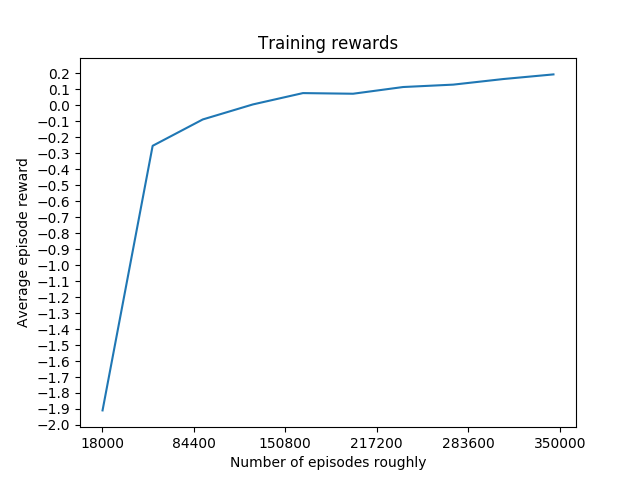
\includegraphics[width=0.65\textwidth]{dql-results.png}
\caption{Deep Q-Learning reward vs. training episodes}
\end{figure}
As seen in the plot, the reward increases at a higher rate at the beginning of training, then increases steadily. After being trained for roughly 350,000 episodes (1,900,000 steps), the agent achieves a reward of 0.194. If trained for more time, the reward will still likely increase, but due to the long training hours, we stopped at 350,000 episodes to see how it performs against the normal Q-agent. After testing for 86,000 episodes, it achieves an average reward of 0.3854, a winning percentage of 16.87\%, and a board completion rate of 42.7\%.
\\\\
Compared with the normal Q-agent, the average reward is generally lower possibly because the deep agent has not yet completely learned to not step on the same cell repeatedly judging from its visualization, receiving negative rewards. Moreover, the normal Q-agent manages to achieve a higher board completion rate. However, one should note that the deep agent is trained for about 23 times fewer episodes within roughly the same amount of time of 8 hours, and still achieves a higher winning percentage. 

\section{Conclusion}

Reward structure is critical in determining the agent’s ability to succeed. Naivety is a danger, but over-complexity can weaken the agent’s policy as well. Comparing Q learning with deep Q learning algorithms, deep Q learning takes more time to train. Trained for the same amount of time, the normal Q agent performs better in terms of average reward and board completion rate, but the deep agent has a higher winning rate. Hence, it is unclear to say one is necessarily better than the other, but it is likely that the deep agent will outperform the normal Q agent if trained for the same amount of episodes, and it is more practical for a larger board. Both the trained normal Q agent and deep agent perform substantially better than the baseline random agent. More generally, Q table suffers from a finite state space, but a deep Q neural net does not since the size of Q table increases substantially as training or board size increases, while the size of weights for a neural net stays relatively stable. 

\subsection{Future Work}

It is likely that given the time, more training will yield better results. There are also a few more hyperparameters to be tuned for deep Q learning:

\begin{itemize}
\item \textbf{target\_model\_update} to determine how often the target copied network should be updated
\item \textbf{nb\_steps\_warmup} to determine how long we wait before actually training the network
\item \textbf{Memory limit} for experience relay
\end{itemize}

Different neural net structures could be experimented more, such as convolutional neural net (CNN) and recurrent neural net (RNN). We did try using CNN but a phenomenon called \emph{catastrophic forgetting} occurred where the agent unlearns its experience in an unexpected way, having initially increasing rewards and then drastically decreasing rewards afterwards. Lastly, an interesting question to ask is: is there a way to utilize the Q table / neural network from smaller boards to be combined to a larger one for a larger board?

\section*{Acknowledgement}

We'd like to thank our professor, Dr. Nishant Mehta, for providing insights when consulted about the project.
\printbibliography[title={References}]
\section*{Appendix A}

Results of experiments with the reward structures with different board sizes. 
\begin{figure}[h]
\centering
\makebox[\textwidth]{
	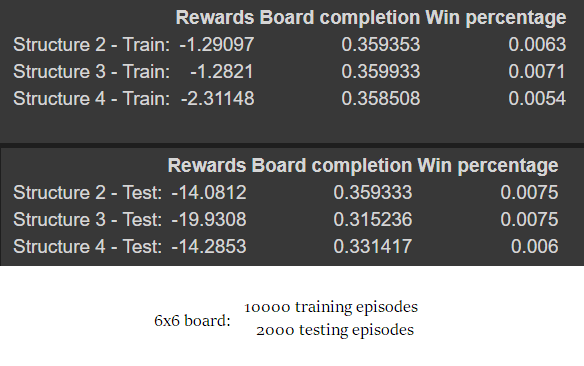
\includegraphics[width=0.55\textwidth]{reward-1.png}
	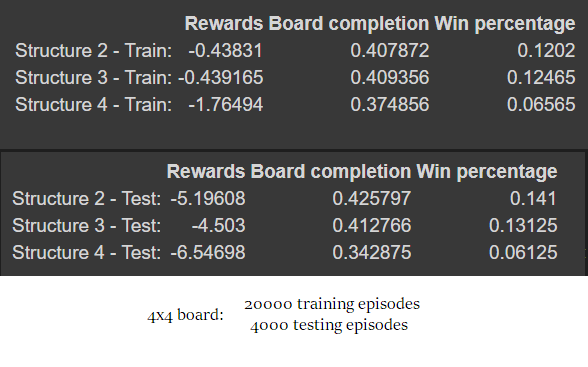
\includegraphics[width=0.55\textwidth]{reward-3.png}
}
\makebox[\textwidth]{
	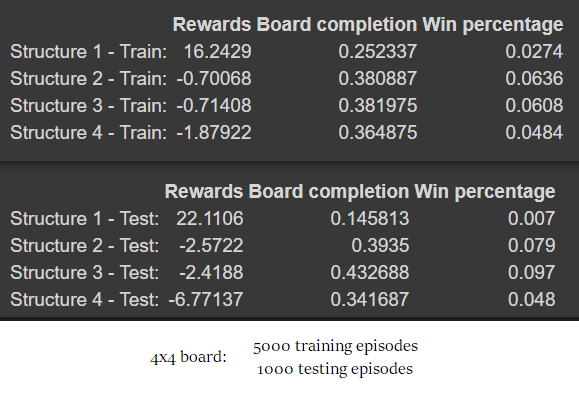
\includegraphics[width=0.55\textwidth]{reward-2.png}
	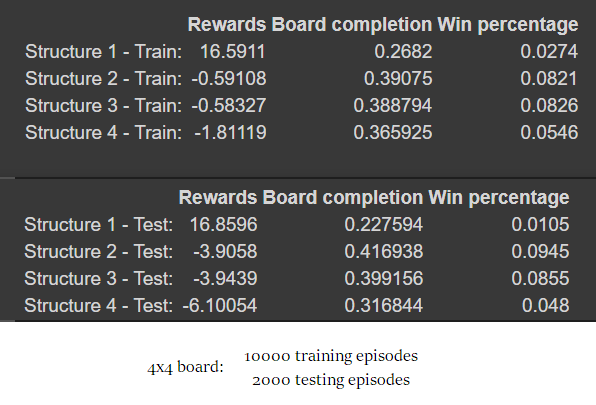
\includegraphics[width=0.55\textwidth]{reward-5.png}
}
\makebox[\textwidth]{
	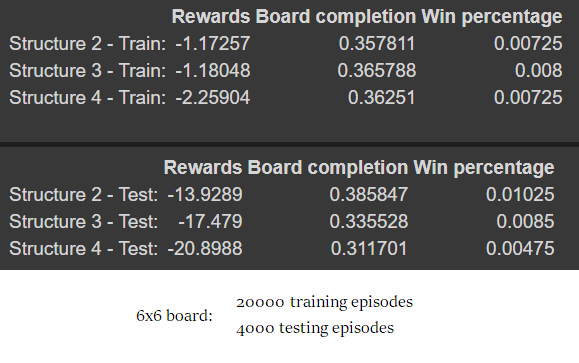
\includegraphics[width=0.55\textwidth]{reward-4.png}
}
\end{figure}

\newpage

\section*{Appendix B}

Score, win percentage, and board completion results from hyperparameter tuning.
\\\\
\textbf{Discount Rate}
\begin{figure}[h]
\centering
\makebox[\textwidth]{
	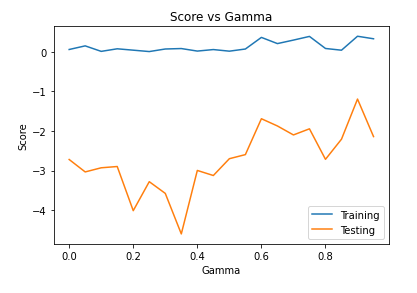
\includegraphics[width=0.4\textwidth]{gamma-score.png}
	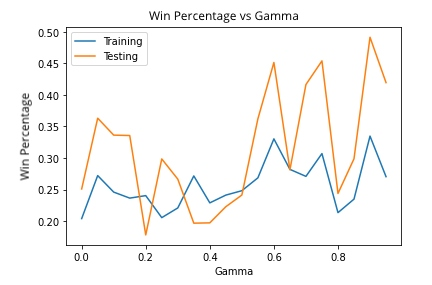
\includegraphics[width=0.4\textwidth]{gamma-win.jpg}
	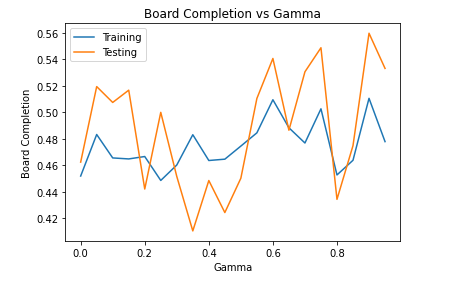
\includegraphics[width=0.4\textwidth]{gamma-board.png}
}
\end{figure}\\
\textbf{Learning Rate}
\begin{figure}[h]
\makebox[\textwidth]{
	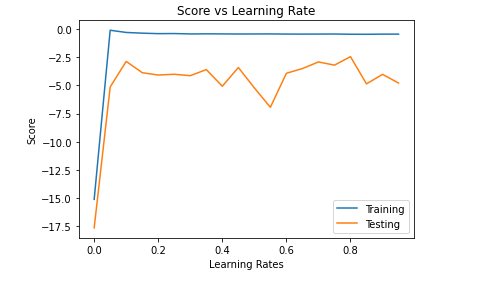
\includegraphics[width=0.4\textwidth]{alpha-score.png}
	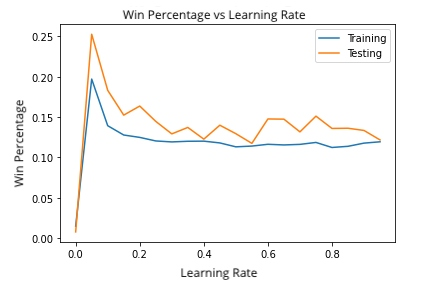
\includegraphics[width=0.4\textwidth]{alpha-win.jpg}
	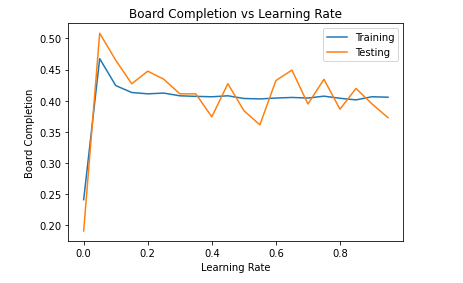
\includegraphics[width=0.4\textwidth]{alpha-board.png}
}
\end{figure}\\
\textbf{Minimum Exploration Rate}
\begin{figure}[h]
\makebox[\textwidth]{
	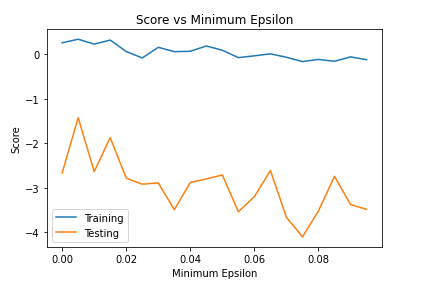
\includegraphics[width=0.4\textwidth]{epsilon-score.png}
	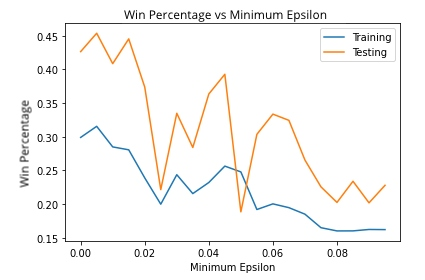
\includegraphics[width=0.4\textwidth]{epsilon-win.jpg}
	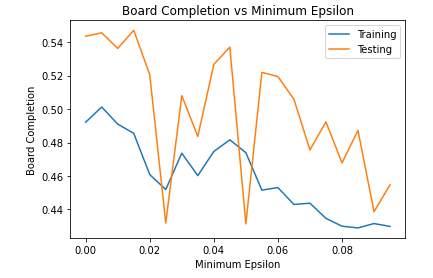
\includegraphics[width=0.4\textwidth]{epsilon-board.png}
}
\end{figure}
\newpage
\textbf{Exploration Decay Rate}
\begin{figure}[h]
\makebox[\textwidth]{
	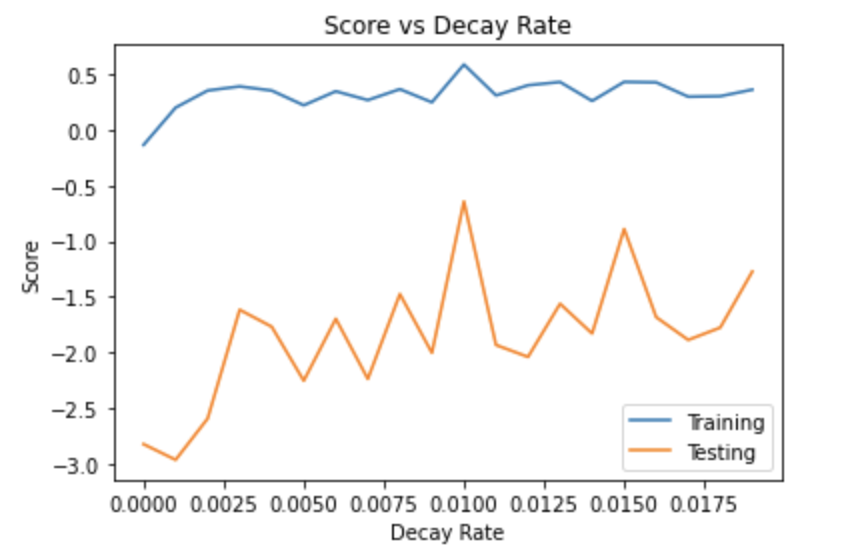
\includegraphics[width=0.4\textwidth]{decay-score.png}
	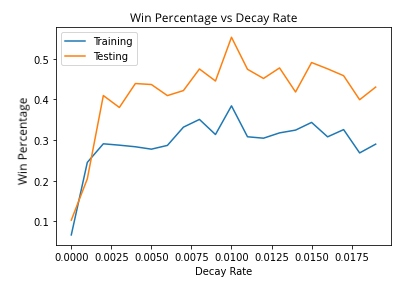
\includegraphics[width=0.4\textwidth]{decay-win.jpg}
	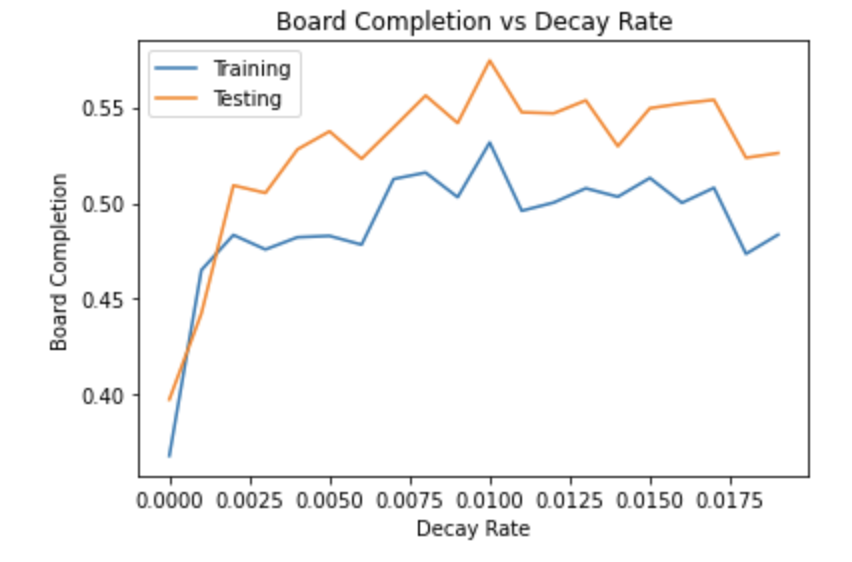
\includegraphics[width=0.4\textwidth]{decay-board.png}
}
\end{figure}

\newpage

\section*{Appendix C}

The 5-layer neural network used for the deep Q-learning agent.

\begin{figure}[h]
\centering
\makebox[\textwidth]{
	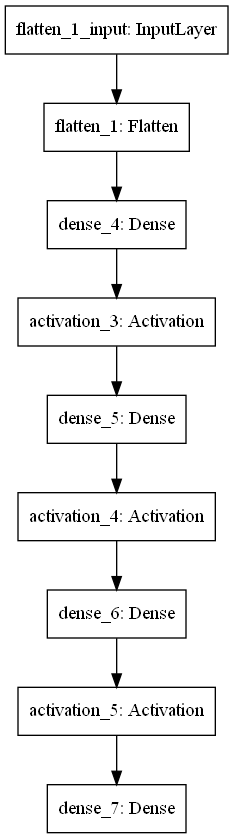
\includegraphics[width=0.3\textwidth]{dql-network.png}
}
\end{figure}
\end{document}
